\begin{enumerate}[(a)]
\item \textbf{\underline{Collet’s Approach for Model Selection:}}. First we import the data into \verb|R| and have a look at the variables of interest.
\begin{spacing}{1.2}
\begin{footnotesize}
\begin{verbatim}
> ###################################################
> ### LAB 6: Model Selection in Survival Analysis ###
> ###################################################
> 
> # (a): Collet’s Approach for Model Selection:
> mac <- read.csv("C:/Applied_Survival_Analysis_Jan2016/lab6/data/mac.csv")
> 
> # The variables we're interested in are:
> vars = c("agecat","sex","cd4","karnof","ivdrug","antiret","rif","clari")
> 
> # Note that in this lab we're focusing on time to death
> mac[1:5,c("dthtime","dthstat",vars)]
  dthtime dthstat agecat sex cd4 karnof ivdrug antiret rif clari
1     623       0      1   0   8     90      0       1   1     0
2     651       0      0   0  30     90      0       0   1     0
3     464       1      1   0  80    100      0       1   1     0
4     622       0      0   0  58     80      0       0   0     1
5     643       0      1   0  59     90      0       0   0     1
\end{verbatim}
\end{footnotesize}
\end{spacing}
Please, see the previous lab to see how treatment type is coded. 
\begin{enumerate}[Step 1:]
\item To facilitate the analysis, we're going to create the formulas required in \verb|coxph| for each variable of interest. For example, let's see the formula for \emph{agecat}
\begin{spacing}{1.2}
\begin{footnotesize}
\begin{verbatim}
> #####################################################################
> ### Step 1: Fit univariate models to choose candidate predictors. ###
> ### Use criterion of p <= 0.15 to identify predictors.            ###
> #####################################################################
> 
> time.expr = "Surv(dthtime,dthstat) ~ "
> 
> # See what's happening here
> paste(time.expr,vars[1])
[1] "Surv(dthtime,dthstat) ~  agecat"
> formula(paste(time.expr,vars[1]))
Surv(dthtime, dthstat) ~ agecat
\end{verbatim}
\end{footnotesize}
\end{spacing}
Note that the \verb|paste| function here is used to concatenate the strings. Now we're going to get the results for each variable of interest using a \verb|for| loop. We save each model in an object called \verb|fit|. Then we can easily extract all the information we need from this object (see \verb|?coxph.object|, and type \verb|str(fit)| and \verb|str(summary(fit))| to see what's included in \verb|fit|).
\begin{spacing}{1.2}
\begin{footnotesize}
\begin{verbatim}
> # Constructing the Table1
> table1 = data.frame(Estimate = rep(NA,8),SE = NA,Pvalue = NA)
> rownames(table1) = vars
> 
> library(survival)
> for (i in 1:(length(vars)-2))
+ {
+   # Fit univariate models
+   fit = coxph(formula(paste(time.expr,vars[i])),data = mac)
+   
+   # Save results
+   res = summary(fit)
+   
+   table1[i,] = c(coef(fit),sqrt(vcov(fit)),res$logtest[3])
+ }
> 
> # We need both rif and clari to evaluate the treatment effect!
> fit = coxph(Surv(dthtime,dthstat) ~ rif + clari,data = mac)
> res = summary(fit)
> 
> table1[7:8,"Estimate"] = coef(fit)
> table1[7:8,"SE"] = sqrt(diag(vcov(fit)))
> table1[7:8,"Pvalue"] = res$coef[,5]
> table1$HR = exp(table1$Estimate)
> round(table1,3)
        Estimate    SE Pvalue    HR
agecat     0.367 0.093  0.000 1.443
sex        0.236 0.145  0.115 1.266
cd4       -0.012 0.002  0.000 0.988
karnof    -0.045 0.005  0.000 0.956
ivdrug     0.102 0.122  0.408 1.108
antiret   -0.214 0.099  0.033 0.808
rif       -0.087 0.107  0.417 0.916
clari     -0.115 0.108  0.285 0.891
> 
> # Wald test for the combined effect of treatment
> res$waldtest
     test        df    pvalue 
1.2600000 2.0000000 0.5337685 
\end{verbatim}
\end{footnotesize}
\end{spacing}
When evaluating the significance of treatment we must include both the \emph{rif}
and \emph{clari} effects in the model. It seems that the effect of treatment on time to death is not significant.
\newpage
\item \begin{enumerate}[(i)]
\item \begin{spacing}{1.2}
\begin{footnotesize}
\begin{verbatim}
> ######################################################
> ### Step 2 (i): Fit a multivariate model with all  ###
> ### significant predictors (p <= 0.15) from Step 1 ###
> ######################################################
> 
> vars[table1$Pvalue<=0.15]
[1] "agecat"  "sex"     "cd4"     "karnof"  "antiret"
> 
> fitStep2i = coxph(Surv(dthtime,dthstat) ~ agecat + sex + cd4 + karnof 
+                   + antiret,data = mac)
> summary(fitStep2i)
Call:
coxph(formula = Surv(dthtime, dthstat) ~ agecat + sex + cd4 + 
    karnof + antiret, data = mac)

  n= 1177, number of events= 514 

             coef exp(coef)  se(coef)      z Pr(>|z|)    
agecat   0.351471  1.421157  0.093913  3.743 0.000182 ***
sex      0.314488  1.369558  0.146148  2.152 0.031409 *  
cd4     -0.010521  0.989534  0.001558 -6.751 1.47e-11 ***
karnof  -0.038088  0.962628  0.005101 -7.467 8.19e-14 ***
antiret -0.232397  0.792631  0.099217 -2.342 0.019165 *  
---
Signif. codes:  0 ‘***’ 0.001 ‘**’ 0.01 ‘*’ 0.05 ‘.’ 0.1 ‘ ’ 1

        exp(coef) exp(-coef) lower .95 upper .95
agecat     1.4212     0.7037    1.1822    1.7084
sex        1.3696     0.7302    1.0284    1.8238
cd4        0.9895     1.0106    0.9865    0.9926
karnof     0.9626     1.0388    0.9531    0.9723
antiret    0.7926     1.2616    0.6526    0.9628

Concordance= 0.663  (se = 0.013 )
Rsquare= 0.12   (max possible= 0.997 )
Likelihood ratio test= 149.9  on 5 df,   p=0
Wald test            = 144.4  on 5 df,   p=0
Score (logrank) test = 145.8  on 5 df,   p=0
\end{verbatim}
\end{footnotesize}
\end{spacing}
\item It seems that there is no function implementing stepwise regression based on p-values in \verb|R|. However, we can use the \verb|stepAIC| function of the library \verb|MASS| instead, which carries out stepwise procedure based on the \emph{AIC} criterion and works for \verb|coxph| objects. Recall that given a set of candidate models for the data, the preferred model is the one with the minimum \emph{AIC} value. Hence \emph{AIC} rewards goodness of fit (as assessed by the likelihood function), but it also includes a penalty that is an increasing function of the number of estimated parameters. This penalty discourages overfitting.

The outline of stepwise procedures is briefly described below: 
\begin{itemize}
\item \underline{Backward step:} among some variables for elimination from the model, the one that optimizes (through its elimination) the AIC criterion is eliminated; It stops when eliminating another variable would increase AIC.
\item \underline{Forward step:} among some variables for addition to the model, the one that optimizes (through its addition) the AIC criterion is added; It stops when adding another variable would increase AIC.
\item \underline{Stepwise procedure:} It's a combination of both backward and forward steps.
\end{itemize}
Let's have a look at the arguments of \verb|stepAIC|
\begin{spacing}{1.2}
\begin{footnotesize}
\begin{verbatim}
> args(stepAIC)
function (object, scope, scale = 0, direction = c("both", "backward", 
    "forward"), trace = 1, keep = NULL, steps = 1000, use.start = FALSE, 
    k = 2, ...) 
\end{verbatim}
\end{footnotesize}
\end{spacing}
This function requires the initial model to be used, and also the minimum and maximum models to be examined. From the help file of \verb|stepAIC|, we get
\begin{spacing}{1.2}
\begin{footnotesize}
\begin{verbatim}
object: an object representing a model of an appropriate class. 
This is used as the initial model in the stepwise search.

scope: defines the range of models examined in the stepwise search. 
This should be either a single formula, 
or a list containing components upper and lower, both formulae. 
See the details for how to specify the formulae and how they are used.
\end{verbatim}
\end{footnotesize}
\end{spacing}
and 
\begin{spacing}{1.2}
\begin{footnotesize}
\begin{verbatim}
Details

The set of models searched is determined by the scope argument. 
The right-hand-side of its lower component is always included in the model, 
and right-hand-side of the model is included in the upper component. 
If scope is a single formula, it specifies the upper component, 
and the lower model is empty. 
If scope is missing, the initial model is used as the upper model.
\end{verbatim}
\end{footnotesize}
\end{spacing}
So, in our case the initial model to be examined should include the variables \emph{agecat}, \emph{sex}, \emph{cd4}, \emph{karnof} and \emph{antiret}. The maximum model should be also the same, whereas the minimum model should be the NULL model (i.e, one without covariates). Thus, taking into account the syntax of \verb|stepAIC|, the scope argument is not necessary in this case
\begin{spacing}{1.2}
\begin{footnotesize}
\begin{verbatim}
> # (ii): Use backward selection to eliminate non-significant predictors 
> # in a multivariate  framework using the AIC criterion
> # Type install.packages("MASS") if needed
> library(MASS)
> fitStep2ii = stepAIC(fitStep2i, direction = "backward", k = 3,trace = 10)
Start:  AIC=6650.94
Surv(dthtime, dthstat) ~ agecat + sex + cd4 + karnof + antiret

trying - agecat
trying - sex
trying - cd4
trying - karnof
trying - antiret
          Df    AIC
<none>       6650.9
- sex      1 6652.2
- antiret  1 6653.2
- agecat   1 6662.4
- karnof   1 6701.2
- cd4      1 6702.3
\end{verbatim}
\end{footnotesize}
\end{spacing}
Note that the choice of \verb|k=3| in the calculation of \emph{AIC} is roughly equivalent to using a 5\% significance level in a likelihood ratio test that compares two nested models which differ by between one and three parameters (see section 3.6.1 in Collet). We can see that there is no variable eliminated from the model, as each elimination leads to an increased value of \emph{AIC}.
\end{enumerate}
\item The multivariate 
model obtained at the end of Step 2 includes the variables \emph{agecat}, \emph{sex}, \emph{cd4}, \emph{karnof} and \emph{antiret}. Thus, at this stage, we have to re-examine the significance of variables \emph{ivdrug}, \emph{rif} and \emph{clari}, which failed to be significant at Step 1. Here, we need to use the argument \verb|scope| in order to force the variables \emph{agecat}, \emph{sex}, \emph{cd4}, \emph{karnof} and \emph{antiret} into the model. 
Moreover, be careful, as the \verb|stepAIC| function examines the significance of each independent variable separately, thus it does not take into account the fact that the variables \emph{rif} and \emph{clari} are both referring to the treatment effect. To properly investigate the treatment effect, we have to create a \verb|factor| containing the treatment groups 
\begin{spacing}{1.2}
\begin{footnotesize}
\begin{verbatim}
> ##########################################################################
> ### Step 3: Use forward selection to add any variables not significant ###
> ### at Step 1 to the multivariate model obtained at the end of Step 2  ###                     
> ##########################################################################
> 
> # Force the variables that are significant at the end of Step 2 into the model,
> # by using the scope argument i.e.,
> # tell R which is the minimum and maximum possible model to be examined
> 
> # To evaluate the signifance of treatment jointly, 
> # you must create a factor with the treatment arms
> trt = rep(NA,nrow(mac))
> trt[mac$rif==1] = "rif"
> trt[mac$clari==1] = "clari"
> trt[mac$rif==0 & mac$clari==0] = "both"
> trt = factor(trt,levels = c("both","rif","clari"))
> mac$trt = trt
> 
> max.model = formula(Surv(dthtime,dthstat) ~ agecat + sex + cd4 + karnof + 
+                       ivdrug + antiret + trt)
> 
> fitStep3=stepAIC(fitStep2i,
+                  scope=list(lower = formula(fitStep2i),upper = max.model),
+                  k = 3,trace = 10,direction = "forward")
Start:  AIC=6650.94
Surv(dthtime, dthstat) ~ agecat + sex + cd4 + karnof + antiret

trying + ivdrug
trying + trt
         Df    AIC
<none>      6650.9
+ ivdrug  1 6653.5
+ trt     2 6656.3
\end{verbatim}
\end{footnotesize}
\end{spacing}
There is no variable added in the model.
\item \begin{enumerate}[(i)]
\item Here, we would like to carry out a \textbf{forward} stepwise procedure including the variables \emph{agecat}, \emph{sex}, \emph{cd4}, \emph{karnof}, \emph{antiret} (full model). To perform such a procedure, we have to tell R to start with the null model and search through models lying in the
range between the null and full model
\begin{spacing}{1.2}
\begin{footnotesize}
\begin{verbatim}
> ########################################################################
> ### Step 4: (i) Do final pruning of main-effects model using forward ###        
> ### forward stepwise regression                                      ###                           
> ########################################################################
> 
> # Starting model (NULL model)
> fit = coxph(Surv(dthtime,dthstat) ~ 1,data = mac)
> 
> fitStep4i = stepAIC(fit,
+                  scope=list(lower = formula(fit),upper = formula(fitStep2i)),
+                  k = 3,trace = 10,direction = "both")
Start:  AIC=6785.88
Surv(dthtime, dthstat) ~ 1

trying + agecat
trying + sex
trying + cd4
trying + karnof
trying + antiret
          Df    AIC
+ karnof   1 6712.1
+ cd4      1 6721.9
+ agecat   1 6772.8
+ antiret  1 6784.3
<none>       6785.9
+ sex      1 6786.4

Step:  AIC=6712.06
Surv(dthtime, dthstat) ~ karnof

trying - karnof
trying + agecat
trying + sex
trying + cd4
trying + antiret
          Df    AIC
+ cd4      1 6665.4
+ agecat   1 6704.7
+ antiret  1 6710.0
<none>       6712.1
+ sex      1 6712.6
- karnof   1 6785.9

Step:  AIC=6665.35
Surv(dthtime, dthstat) ~ karnof + cd4

trying - karnof
trying - cd4
trying + agecat
trying + sex
trying + antiret
          Df    AIC
+ agecat   1 6653.8
+ antiret  1 6662.8
<none>       6665.4
+ sex      1 6665.6
- cd4      1 6712.1
- karnof   1 6721.9

Step:  AIC=6653.81
Surv(dthtime, dthstat) ~ karnof + cd4 + agecat

trying - karnof
trying - cd4
trying - agecat
trying + sex
trying + antiret
          Df    AIC
+ antiret  1 6652.2
+ sex      1 6653.2
<none>       6653.8
- agecat   1 6665.4
- karnof   1 6703.6
- cd4      1 6704.7

Step:  AIC=6652.21
Surv(dthtime, dthstat) ~ karnof + cd4 + agecat + antiret

trying - karnof
trying - cd4
trying - agecat
trying - antiret
trying + sex
          Df    AIC
+ sex      1 6650.9
<none>       6652.2
- antiret  1 6653.8
- agecat   1 6662.8
- karnof   1 6702.6
- cd4      1 6703.3

Step:  AIC=6650.94
Surv(dthtime, dthstat) ~ karnof + cd4 + agecat + antiret + sex

trying - karnof
trying - cd4
trying - agecat
trying - antiret
trying - sex
          Df    AIC
<none>       6650.9
- sex      1 6652.2
- antiret  1 6653.2
- agecat   1 6662.4
- karnof   1 6701.2
- cd4      1 6702.3
Warning messages:
1: In is.na(fit$coefficients) :
  is.na() applied to non-(list or vector) of type 'NULL'
2: In is.na(fit$coefficients) :
  is.na() applied to non-(list or vector) of type 'NULL'
3: In is.na(fit$coefficients) :
  is.na() applied to non-(list or vector) of type 'NULL'
4: In is.na(fit$coefficients) :
  is.na() applied to non-(list or vector) of type 'NULL'
\end{verbatim}
\end{footnotesize}
\end{spacing}
Note that by using the option \verb|trace = 10| we can see each step of the procedure in detail. Please, make sure you understand the way the algorithm works. At the first step, the karnofsky score status is added to the model because it has the best effect on the \emph{AIC} criterion. Then, CD4 is added to the model including the karnofsky score. However, both variables can be eliminated from the model at the next steps. Finally, we ended up with the full model, i.e., all variables were added to the model.  
\item Now, we consider adding interactions of the main effects of our last model. We are going to use a \textbf{backward} stepwise procedure to check if there are any significant interaction terms under the hierarchical principle. To do so, we must force the main effects into the model by defining the minimum model to be the one that includes all the main effects. Thus,
\begin{spacing}{1.2}
\begin{footnotesize}
\begin{verbatim}
> # (ii) Adding interaction terms
> mac$agsex = mac$agecat*mac$sex 
> mac$agcd4 = mac$agecat*mac$cd4 
> mac$agkar = mac$agecat*mac$karnof 
> mac$aganti = mac$agecat*mac$antiret 
> mac$sexcd4 = mac$sex*mac$cd4 
> mac$sexkar = mac$sex*mac$karnof 
> mac$sexanti = mac$sex*mac$antiret 
> mac$cd4kar = mac$cd4*mac$karnof 
> mac$cd4anti = mac$cd4*mac$antiret 
> mac$karanti = mac$karnof*mac$antiret
> 
> max.model = formula(Surv(dthtime,dthstat) ~ agecat + sex + cd4 + karnof 
+                     + antiret + agsex 
+                     + agcd4 + agkar + aganti + sexcd4 + sexkar + sexanti 
+                     + cd4kar + cd4anti + karanti)
> 
> # Fit the maximum model
> fit = coxph(max.model,data = mac)
> 
> fitStep4ii = stepAIC(fit,
+                      scope = list(lower = formula(fitStep2i),upper = max.model),
+                    k = 3,trace = 0,direction = "both")
> fitStep4ii$anova
Stepwise Model Path 
Analysis of Deviance Table

Initial Model:
Surv(dthtime, dthstat) ~ agecat + sex + cd4 + karnof + antiret + 
    agsex + agcd4 + agkar + aganti + sexcd4 + sexkar + sexanti + 
    cd4kar + cd4anti + karanti

Final Model:
Surv(dthtime, dthstat) ~ agecat + sex + cd4 + karnof + antiret + 
    sexanti + karanti


       Step Df  Deviance Resid. Df Resid. Dev      AIC
1                             1162   6622.959 6667.959
2  - sexkar  1 0.1823756      1163   6623.142 6665.142
3 - cd4anti  1 0.1664674      1164   6623.308 6662.308
4   - agkar  1 0.2457168      1165   6623.554 6659.554
5  - sexcd4  1 0.6021998      1166   6624.156 6657.156
6   - agsex  1 0.5886611      1167   6624.745 6654.745
7  - aganti  1 0.6292394      1168   6625.374 6652.374
8   - agcd4  1 0.7502989      1169   6626.124 6650.124
9  - cd4kar  1 1.6707913      1170   6627.795 6648.795
\end{verbatim}
\end{footnotesize}
\end{spacing}
Note that since we want to carry out a backward procedure, we started with the full model. The interaction terms of antiretroviral therapy with the karnofsky score and sex were finally added in the model.
\end{enumerate}
\item Based on our last model we consider
\begin{enumerate}[(i)] 
\item \emph{cd4cat} instead of \emph{cd4}
\begin{spacing}{1.2}
\begin{footnotesize}
\begin{verbatim}
> ##############################################
> ### Step 5: alternate coding of covariates ###
> ##############################################
> 
> # See the formula of the last model
> formula(fitStep4ii)
Surv(dthtime, dthstat) ~ agecat + sex + cd4 + karnof + antiret + 
    sexanti + karanti
> 
> # (i): cd4cat instead of cd4
> fitStep5i = coxph(Surv(dthtime, dthstat) ~ agecat + sex + cd4cat + 
+                     karnof + antiret + sexanti + karanti,data = mac)
\end{verbatim}
\end{footnotesize}
\end{spacing}
\item \emph{age} instead of \emph{agecat}
\begin{spacing}{1.2}
\begin{footnotesize}
\begin{verbatim}
> # (ii): age instead of agecat
> fitStep5ii = coxph(Surv(dthtime, dthstat) ~ age + sex + cd4 + karnof 
+                    + antiret + sexanti + karanti,data = mac)
\end{verbatim}
\end{footnotesize}
\end{spacing}
\end{enumerate}
\item Note that our models have been saved in the objects \emph{fitStep2i},  \emph{fitStep2ii}, \emph{fitStep3}, \emph{fitStep4i}, \emph{fitStep4ii}, \emph{fitStep5i} and \emph{fitStep5ii}. So, we can easily extract the \emph{AIC} criterion from these objects using the \verb|extractAIC| function.
\begin{spacing}{1.2}
\begin{footnotesize}
\begin{verbatim}
> # Summarize the results in a table
> models = data.frame(Model = c("Step 2 (i)","Step 2 (ii)","Step 3","Step 4 (i)",
+                               "Step 4 (ii)","Step 5 (i)","Step 5 (ii)"),
+                     Covariates = NA,twlogl = NA,q = NA,AIC = NA)
> 
> md = c("fitStep2i","fitStep2ii","fitStep3","fitStep4i",
+        "fitStep4ii","fitStep5i","fitStep5ii")
> 
> for (i in 1:7)
+ {
+   obj = get(md[i])
+   models[i,2] = paste(names(coef(obj)),collapse = " ")
+   models[i,-(1:2)] = c(-2*obj$logl[2],extractAIC(obj,k=3))
+ }
> 
> models
        Model                                       Covariates   twlogl q      AIC
1  Step 2 (i)                    agecat sex cd4 karnof antiret 6635.938 5 6650.938
2 Step 2 (ii)                    agecat sex cd4 karnof antiret 6635.938 5 6650.938
3      Step 3                    agecat sex cd4 karnof antiret 6635.938 5 6650.938
4  Step 4 (i)                    karnof cd4 agecat antiret sex 6635.938 5 6650.938
5 Step 4 (ii)    agecat sex cd4 karnof antiret sexanti karanti 6627.795 7 6648.795
6  Step 5 (i) agecat sex cd4cat karnof antiret sexanti karanti 6644.395 7 6665.395
7 Step 5 (ii)       age sex cd4 karnof antiret sexanti karanti 6625.956 7 6646.956
\end{verbatim}
\end{footnotesize}
\end{spacing}
According to the \emph{AIC} criterion the best model is the model in Step 5 (ii), the one with the 
smallest \emph{AIC}.
\end{enumerate}
\item \textbf{\underline{Assessing Overall Model Fit:}} We first fit the model that includes the variables \emph{age}, \emph{sex}, \emph{cd4}, \emph{karnof} and \emph{antiret}
\begin{enumerate}[(i)]
\item \textbf{Derivation of Cox-Snell residuals:} If $T_{i}$ (the survival time for the $i$th individual) has a survival function $S_{i}(t)$, then the transformed random variable $S_{i}(T_{i})$ (i.e., the survival function evaluated at the actual survival time $T_{i}$) should be a uniform distribution on $[0,1]$, and hence $\Lambda(T_{i})= -\log S_{i}(T_{i})$ should be a unit exponential distribution.

More mathematically,
\begin{align}
\text{If}\quad T_{i} &\sim S_{i}(t) \nonumber \\
\text{Then}\quad S_{i}(T_{i}) &\sim \mathcal{U}(0,1) \nonumber \\
\text{and}\quad -\log S_{i}(T_{i}) &\sim \operatorname{Exp}(1) \label{csnell}
\end{align}
The quantity $r_{CS,i}=\hat{\Lambda}(t_{i}|\mathbf{z}_{i})=\hat{\Lambda}_{0}(t_{i})e^{\mathbf{z}_{i}^{T}\hat{\boldsymbol{\beta}}}
$ is the estimated cumulative hazard for $i$th individual at the time of their death or censoring, and it's called the Cox-Snell residual. The implication of \eqref{csnell} is that the Cox-Snell residuals should be like a censored sample from a unit exponential. Thus, to check if the distribution of the Cox-Snell residuals looks like a unit exponential, we should take censoring into account defining a survival dataset with the Cox-Snell residuals as the
“pseudo” failure times. Then, we can estimate the KM survival of the Cox-Snell residuals $\hat{S}_{CS}(t)$. Based on the properties of a unit exponential distribution
\begin{align}
S(t) = e^{-t} \Rightarrow \log\left[-\log S(t)\right] = \log(t), \nonumber
\end{align}
plotting $\log\left[-\log \hat{S}_{CS}(t)\right]$ vs $\log(t)$ should yield a straight line
through the origin with slope = 1. Be extremely cautious here, as $\hat{S}_{CS}(t)$ denotes the estimated “survival” function of the Cox-Snell residuals \textbf{not} of the original event times! Please, also note that the time scale used on these graphs is the Cox-Snell residuals. Thus,
\begin{spacing}{1.2}
\begin{footnotesize}
\begin{verbatim}
> #################################################
> ### Assessing the overall fit of the model by ###
> ### checking the residuals                    ###
> #################################################
> 
> fit = coxph(Surv(dthtime, dthstat) ~ age + sex + cd4 + karnof + antiret,data = mac)
> #summary(fit)
> 
> # (b)-(i): Generalized (Cox-Snell) Residuals
> mac$csres = mac$dthstat - residuals(fit,type = "martingale")
> 
> setwd("C:/Applied_Survival_Analysis_Jan2016/lab6/graphs")
> 
> pdf("Surv_coxsnell.pdf",height = 5,width = 5)
> fitcs = survfit(Surv(csres,dthstat)~1,data = mac)
> plot(fitcs,fun = "cloglog",conf.int = F,mark.time = F, 
+      xlab = "Cox-Snell residuals (log scale)",ylab = "Log(-log Scs)")
> abline(h = 0,col = "red")
> abline(v = 1,col = "red") # Don't forget the log scale!
> dev.off()
\end{verbatim}
\end{footnotesize}
\end{spacing}
\begin{figure}[htbp]
	\centering
		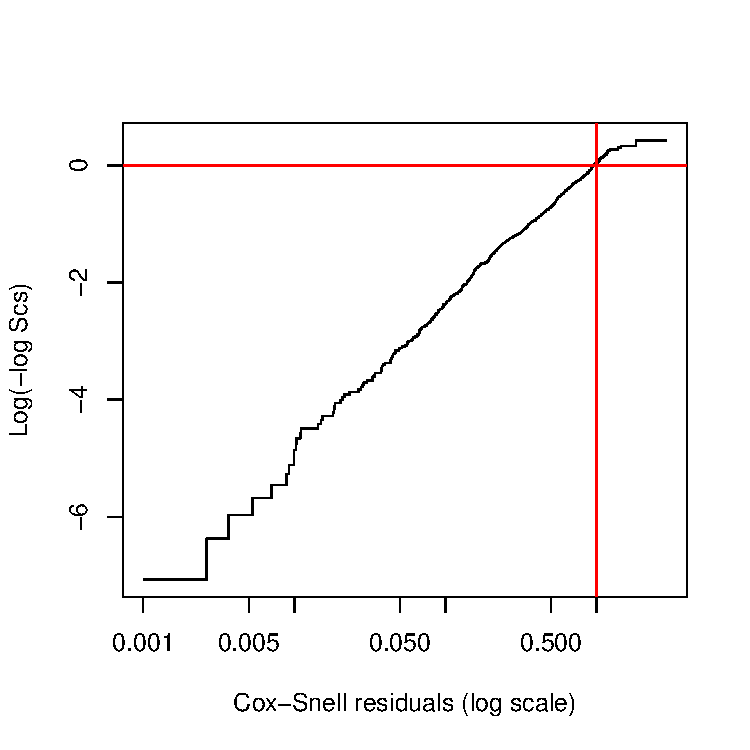
\includegraphics[scale=0.9]{Surv_coxsnell.pdf}
		%\rule{35em}{0.5pt}
	\caption{\emph{log-log} transformed survival function of Cox-Snell residuals .}
	\label{figure1}
\end{figure}
If the model fits the data well, we will expect a straight line. The curve seems fairly linear. However, some further comments on Cox-Snell residuals should be made.
\begin{itemize}
\item Cox-Snell residuals are most useful for
examining overall fit of a model.
\item Such plots can't indicate the type of departure from the
model when the points are not linear.
\item Closeness of the distribution of the residuals to the
unit exponential depends on $n$.
\item Since we plug in the estimated regression
coefficients, departures from the exponential
distribution may be due to the uncertainty in
estimating $\boldsymbol{\beta}$ and $\Lambda_{0}$
\end{itemize}
\item Martingale residuals are defined for the $i$th individual as
\begin{align}
r_{M,i} = \delta_{i} - \hat{\Lambda}(t_{i}|\mathbf{z}_{i}). \nonumber
\end{align}
It can be shown that the expected value of $\delta_{i}$ is $\Lambda(t_{i}|\mathbf{z}_{i})$. Thus, $r_{M,i}$'s have mean 0 and they are like “observed” minus “expected”. However, since their range is between $-\infty$ and 1, they tend to be quite asymmetric in practice. 

In \verb|R|, once an \verb|coxph| is saved, we can easily get the Martingale residuals using the \verb|residuals| function. Please, see \verb|?residuals.coxph| for more details. Also, to compute the linear predictor (i.e., $\mathbf{z}_{i}^{T}\hat{\boldsymbol{\beta}}$), we can use the function \verb|predict| (see \verb|?predict.coxph|).  
\begin{figure}[htbp]
	\centering
		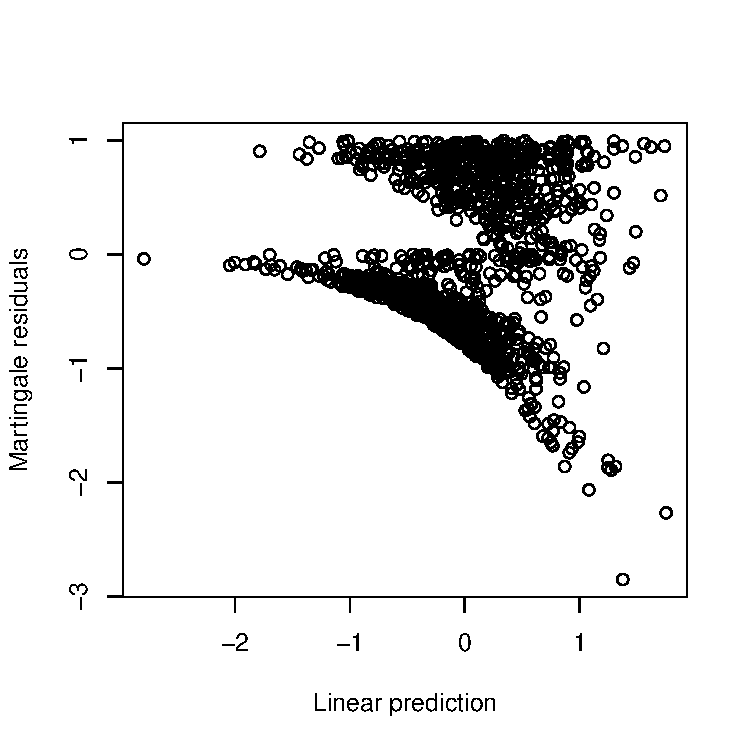
\includegraphics[scale=0.9]{mgale.pdf}
		%\rule{35em}{0.5pt}
	\caption{Martingale residuals vs linear prediction.}
	\label{figure2}
\end{figure}
\begin{spacing}{1.2}
\begin{footnotesize}
\begin{verbatim}
> # b-(ii): Martingale Residuals
> mac$mg = residuals(fit,type = "martingale")
> mac$betaz = predict(fit,type = "lp")
> 
> pdf("mgale.pdf",height = 5,width = 5)
> plot(mg ~ betaz,data = mac,xlab = "Linear prediction",
+      ylab = "Martingale residuals")
> dev.off()
\end{verbatim}
\end{footnotesize}
\end{spacing}
\item While martingale residuals are uncorrelated
and have mean zero, their disadvantage is that:
\begin{itemize}
\item max is +1, but minimum is $-\infty$
\item it's difficult to identify outliers based on them due to their heavily skewed distribution. 
\end{itemize}

That's the reason we have the deviance residuals. They are called “deviance” because they are defined similarly to the deviance residuals in GLMs.
To get them in \verb|R|, we can use the \verb|residuals| function again
\begin{spacing}{1.2}
\begin{footnotesize}
\begin{verbatim}
> # b-(iii): Deviance residuals
> mac$devres = residuals(fit,type = "deviance")
\end{verbatim}
\end{footnotesize}
\end{spacing}
Note that by using the function \verb|par| we can easily combine multiple plots into one overall graph. The option \verb|mfrow=c(nrows, ncols)| creates a matrix of nrows x ncols plots that are filled in by row.
\begin{spacing}{1.2}
\begin{footnotesize}
\begin{verbatim}
> # Deviance residuals vs linear prediction and other covariates
> pdf("devres.pdf",height = 5.5,width = 5.5)
> par(mfrow = c(2,2))
> plot(devres ~ betaz,data = mac,xlab = "Linear prediction",
+      ylab = "Deviance residuals")
> abline(h = 0,col = "red")
> 
> plot(devres ~ age,data = mac,xlab = "Age (years)",
+      ylab = "Deviance residuals")
> abline(h = 0,col = "red")
> 
> plot(devres ~ cd4,data = mac,xlab = "CD4+ cell count",
+      ylab = "Deviance residuals")
> abline(h = 0,col = "red")
> 
> plot(devres ~ karnof,data = mac,xlab = "Karnofsky score status",
+      ylab = "Deviance residuals")
> abline(h = 0,col = "red")
> dev.off()
\end{verbatim}
\end{footnotesize}
\end{spacing}

\begin{figure}
	\centering
		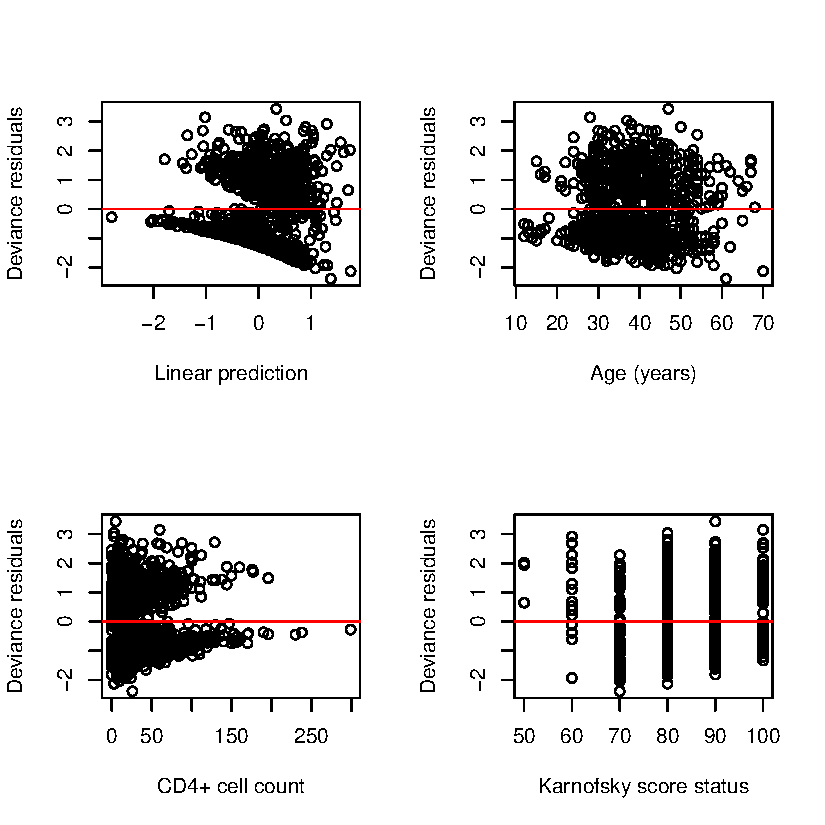
\includegraphics[scale=1]{devres.pdf}
		%\rule{35em}{0.5pt}
	\caption{Deviance residuals vs linear prediction and other covariates.}
	\label{figure3}
\end{figure}
\newpage
\item The Weighted Schoenfeld residuals are defined at each observed failure time for each covariate included in the model. 

\textbf{Key point}: When they are plotted against any transformation $g(t)$ of time $t$, for example, $\log(t)$ or $t$ itself,  the
smooth curve through the plotted points
approximates the manner in which the associated
coefficients depend on time! 

A quick way to obtain the weighted schoenfeld residuals in \verb|R| is using the \verb|cox.zph| function. We also use the option \verb|transform = "identity"| to tell \verb|R| that we don't want to transform the survival times. Note that the \verb|plot| function creates a graph of the scaled Schoenfeld residuals along with a smooth curve when taking a \verb|cox.zph| object as an argument.
\begin{spacing}{1.2}
\begin{footnotesize}
\begin{verbatim}
> # (b)-(iv): Weighted Schoenfeld Residuals
> temp = cox.zph(fit,transform = "identity")
> 
> # Age
> pdf("sclSchAge.pdf",height = 5.5,width = 5.5)
> plot(temp[1],main = "scaled Schoenfeld residuals of Age")
> dev.off()
RStudioGD 
        2 
> 
> # CD4
> pdf("sclSchCd4.pdf",height = 5.5,width = 5.5)
> plot(temp[3],main ="scaled Schoenfeld residuals of CD4")
> dev.off()
RStudioGD 
        2  
\end{verbatim}
\end{footnotesize}
\end{spacing}
Note that we specify the set of variables for which plots are desired through a subscript \verb|[]|.

The fitted smooth curves on the graphs below appear to be roughly horizontal (zero slope), and thus, the proportionality assumption for the age and CD4 effects may be reasonable. Note that we could easily construct a formal test for the PH assumption by fitting a OLS regression line and seeing if the slope is significant (more on the next lecture and lab)!

Some suggestions for the plots of weighted Schoenfeld residuals
\begin{itemize}
\item Try some some different transformations of the survival times, e.g. $g(t)=\log(t)$ or something else (see the options in \verb|cox.zph|)
\item You're advised to perform a sensitivity analysis regarding the parameters of the smoother you're using, and see how the results are changing, especially when the number of events is small (recall that weighted Schoenfeld residuals are defined at event times only).
\end{itemize}

\begin{figure}
	\centering
		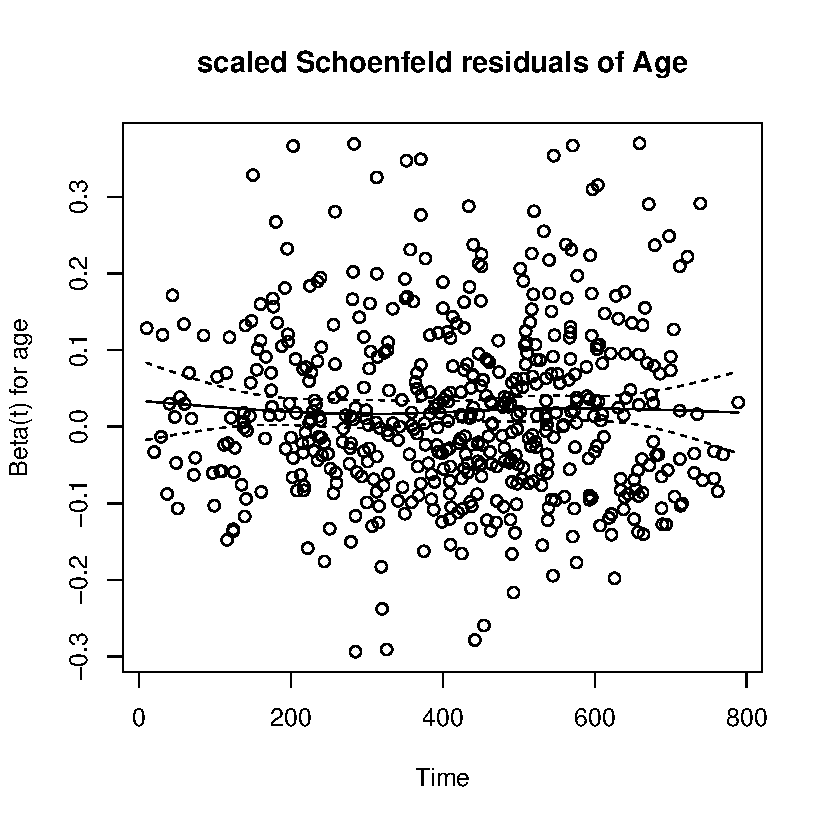
\includegraphics[scale=1]{sclSchAge.pdf}
		%\rule{35em}{0.5pt}
	\caption{Weighted Schoenfeld residuals of age.}
	\label{figure4}
\end{figure}

\begin{figure}
	\centering
		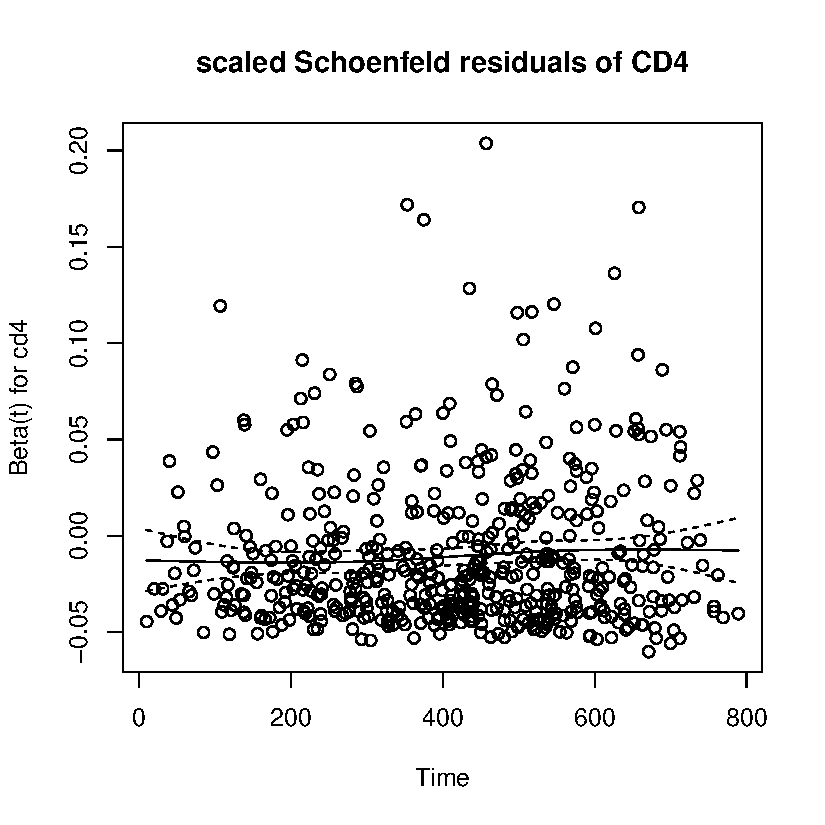
\includegraphics[scale=1]{sclSchCd4.pdf}
		%\rule{35em}{0.5pt}
	\caption{Weighted Schoenfeld residuals of CD4.}
	\label{figure5}
\end{figure}

\item The algorithm seems intuitively reasonable since we have the residuals of the survival time that do not depend on CD4 on the y-axis, whereas the residuals of CD4 after taking into account the other covariates are plotted on the x-axis. Thus, we hope that such a plot will reveal the relationship of CD4 with the survival times after adjusting for the other variables. This plot is also similar to an \emph{added variable plot} (see more on google).
\begin{spacing}{1.2}
\begin{footnotesize}
\begin{verbatim} 
> # Fit a model without CD4
> coxNoCD4 = coxph(Surv(dthtime, dthstat) ~ age + sex + karnof + antiret,data = mac)
> mac$mgNoCD4 = residuals(coxNoCD4,type = "martingale")
> 
> # Regress CD4 on the other covariates
> lmCD4 = lm(cd4 ~ age + sex + karnof + antiret,data = mac)
> mac$CD4res = lmCD4$res
> 
> pdf("funCD4.pdf",height = 5.5,width = 5.5)
> plot(mgNoCD4 ~ CD4res,data = mac, ylab = "CD4-free martingale residuals",
+      xlab = "CD4 residuals")
> lines(smooth.spline(mac$CD4res, mac$mgNoCD4, df = 4), col = "red", lwd = 2)
> dev.off()
\end{verbatim}
\end{footnotesize}
\end{spacing}

\begin{figure}[htbp]
	\centering
		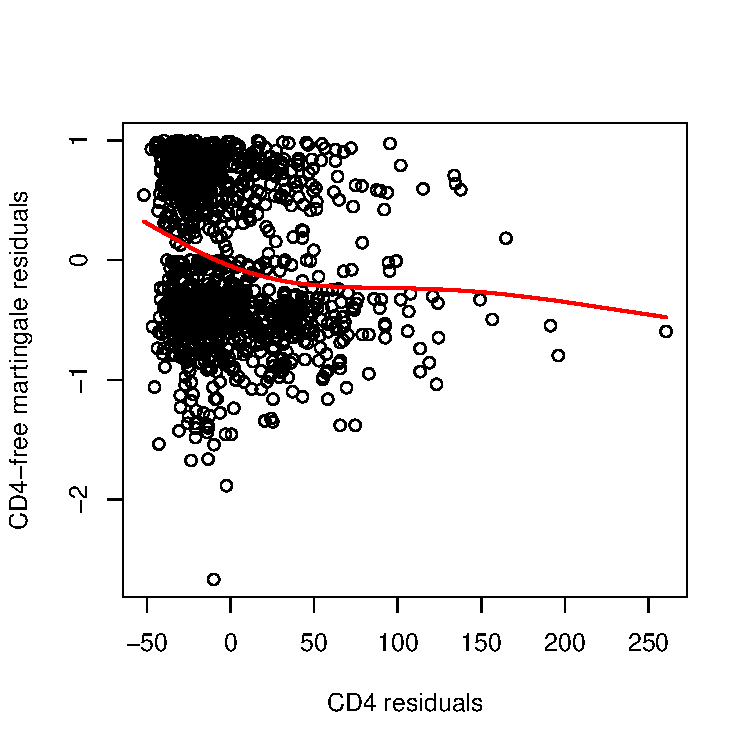
\includegraphics[scale=0.9]{funCD4.pdf}
		%\rule{35em}{0.5pt}
	\caption{Investigating the correct functional form of CD4.}
	\label{figure6}
\end{figure}
In the beginning the relationship appears linear but then it curves, so it does not seem likely that CD4 has a linear effect on the logarithm of the hazard ratio. 

We could apply the square root transformation, which is a very popular transformation of CD4 in the analysis of longitudinal data as it normalizes the distribution and does not have any problem with zeros. 

\begin{spacing}{1.2}
\begin{footnotesize}
\begin{verbatim} 
> # Try sqrt(CD4), very popular transformation in longitudinal data analysis!
> mac$sqCD4res = lm(I(sqrt(cd4)) ~ age + sex + karnof + antiret,data = mac)$res
> 
> pdf("funsqCD4.pdf",height = 5.0,width = 5.0)
> plot(mgNoCD4 ~ sqCD4res,data = mac, ylab = "sqrt(CD4)-free martingale residuals",
+      xlab = "sqrt(CD4) residuals")
> lines(smooth.spline(mac$sqCD4res, mac$mgNoCD4, df = 4), col = "red", lwd = 2)
> dev.off()
\end{verbatim}
\end{footnotesize}
\end{spacing}

\begin{figure}[htbp]
	\centering
		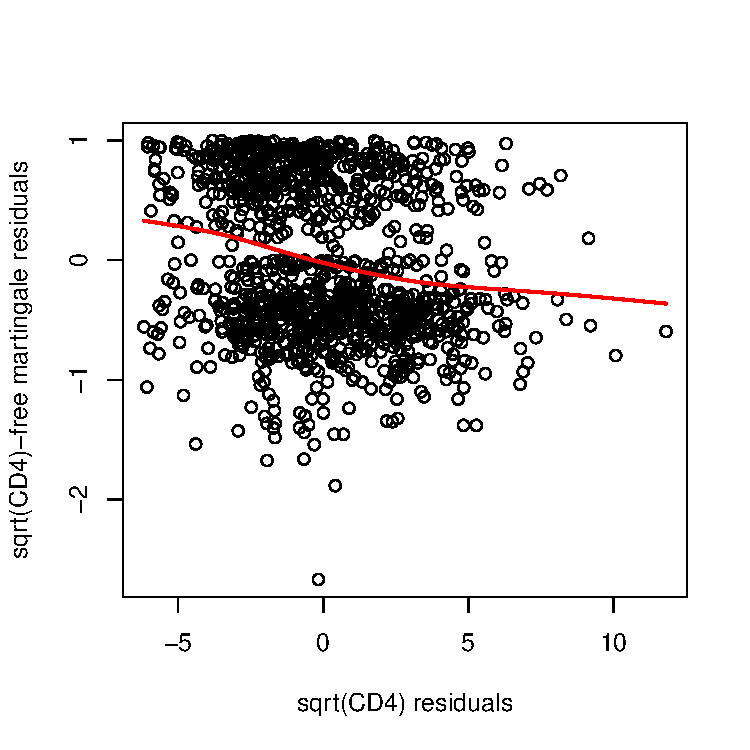
\includegraphics[scale=0.9]{funsqCD4.pdf}
		%\rule{35em}{0.5pt}
	\caption{Investigating the correct functional form of CD4.}
	\label{figure7}
\end{figure}
The linearity assumption seems more plausible on the square root CD4 scale. You can also check if the \emph{AIC} criterion improves by including the square root CD4 values instead of the untransformed ones in the cox model.


\end{enumerate}
\end{enumerate}